%%%%%%%%%%%%%%%%%%%%%%%%%%%%%%%%%%%%%%%%%%%%%%%%%%%%%%%%%%%%%%%%%%%%%%%%%%%%%%%%%%%%%%%%%%%
%                               My System 24pp
%%%%%%%%%%%%%%%%%%%%%%%%%%%%%%%%%%%%%%%%%%%%%%%%%%%%%%%%%%%%%%%%%%%%%%%%%%%%%%%%%%%%%%%%%%%
\chapter{Architecture}
\label{sec:Architecture}
 
\section*{Summary}
 
In this section, we will present our proposal which will be divided as follows. 
In the first place, in section \ref{section-approach-main-objectives} we explain
our goals in detail and what we consider to be an innovation. 
Next, section \ref{section-approach-architecture} will present the planned architecture with a step-by-step 
explanation for the reader to fully understand the desired work flow.
The final section will list the tools that we plan to use in the implementation of our approach.

\subsection{Main Objectives}
\label{section-approach-main-objectives}

Hereby, we present our proposal in which we aim to further explore the possibilities of multimodal 
feedback applied in a rehabilitation context.

We plan to combine multiple sources of feedback: visual, audio and haptic feedback, 
in order to evaluate how the patient responds to these sources of 
guidance throughout the execution of a given movement. 

To provide a dynamic feedback that constantly reacts to the patient's movements, we will rely on real-time skeleton tracking through a motion capture device.

The use of projection mapping in a rehabilitation environment has not been experimented yet, 
and we have reasons to believe it can bring great benefits to the methods of guidance 
applied to a patient in this kind of rehabilitation systems. If combined with an augmented reality mirror 
and audio or haptic feedback, we will be able to approach the same exercises in different ways in order to evaluate which 
feedback combinations can make the patient understand more clearly the required movements.

To control these feedback sources, a rehabilitation system will be implemented.%\todo{dar nome ao sistema?} 
The system will be capable of manipulating the feedback in order to guide
the patient through a predefined exercise which must be previously learned by the system through demonstration.
This way, the system is only responsible for guiding the patient to a correct execution of the chosen exercise.

We will focus this initial proposal only on exercises related to upper limb movement to simplify the implementation and reduce the number of factors that would need to be taken into account. This way we can experiment more with multimodal feedback and achieve more precise results.


\subsection{Architecture}
\label{section-approach-architecture}

The planned architecture of our proposal is divided into two different parts. 
The first, called \emph{Learning Architecture}, consists of the process for obtaining an exercise model by demonstration for further use.
The second and most important part, called \emph{Teaching Architecture}, concerns the application of the multimodal feedback for another person to recreate the exercise model.


\subsubsection{Learning Architecture}

The first part of our architecture serves the purpose of generating an exercise model which will be used for teaching and guiding exercises' execution.

As we can see in Fig. \ref{fig:learning}, we start by having a \ac{PT} demonstrating the prescribed exercise (1). Through motion capture devices, the \ac{PT} body is tracked during the demonstration and the tracking data is stored in a storage infrastructure.

Then, all the tracking data recorded is sent to the \emph{Exercise Generator Module} (2) in which the data will be sanitized (e.g., remove tracking data whenever the \ac{PT} is not performing the exercise) to be fed into the next step.

Finally, the resulting data will be returned from the \emph{Exercise Generator Module} to an element denoted \emph{Exercise Model} (3), which will consist of modelling all the useful data required to recreate the exercise initially demonstrated by the therapist. 

The generated \emph{Exercise Model} will be the foundation of our Architecture's second part, described hereafter.


%\begin{figure}
%	\centering
%	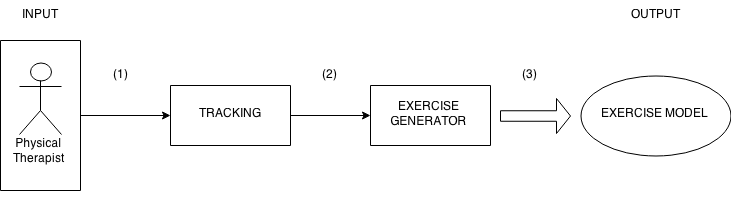
\includegraphics[width=0.8\textwidth]{imgs/LearningPhase}
%	\caption{Learning Architecture Diagram}
%	\label{fig:learning}
%\end{figure}

%\caption{Learning Phase}
\subsubsection{Teaching Architecture}

The second part of our architecture serves the purpose of taking advantage of 
multiple feedback interfaces in order to guide a patient through 
the execution of a previously recorded exercise, the already described \emph{Exercise Model}.

As shown in Fig. \ref{fig:teaching}, it starts by 
loading the desired exercise that was generated in the \emph{Learning Architecture} (4), which will be the basis for comparison with the patient's body.

In this case, the tracking module is responsible for constantly sending the tracking data to the \emph{Multimodal Feedback Manager Module}(MFM) (5,6).

The \ac{MFM} module holds the core of our approach. While receiving real-time tracking data from the patient, the module will compare his current posture to the \emph{Exercise Model}.
With this in mind, the module will communicate (7) with the available feedback interfaces in order to guide the patient, for him to achieve a similar movement to the one recorded.
The module will manipulate each interface independently from one another, to easily create different combinations of feedback so that we can evaluate their validity.
Each one of the three feedback modules available will consist of devices capable of interacting in the desired feedback type: visual, audio or haptic. 

While the patient is still executing the exercise, the required feedback will continue to be applied (8, 9, 10). Therefore, as the patient keeps changing his posture, the tracking data will also be updated and therefore, affecting the resulted feedback.
This process (5-10) will remain in cycle until the given exercise is finished.


%\begin{figure}
%	\centering
%	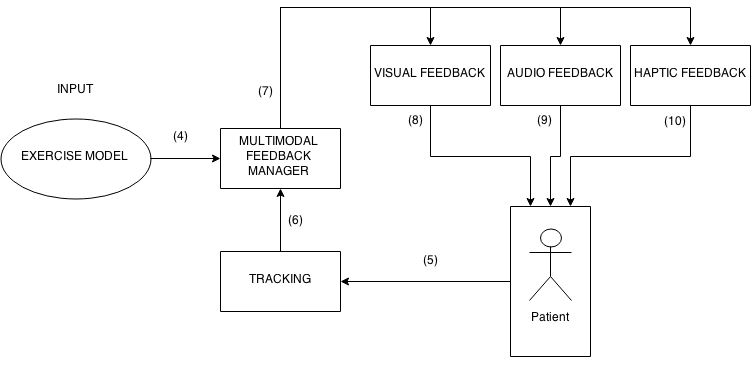
\includegraphics[width=0.8\textwidth]{imgs/TeachingPhase}
%	\caption{Teaching Architecture Diagram}
%	\label{fig:teaching}
%\end{figure}